% This text is proprietary.
% It's a part of presentation made by myself.
% It may not used commercial.
% The noncommercial use such as private and study is free
% Sep. 2005 
% Author: Sascha Frank 
% University Freiburg 
% www.informatik.uni-freiburg.de/~frank/
%
% additional usepackage{beamerthemeshadow} is used
%  
%  \beamersetuncovermixins{\opaqueness<1>{25}}{\opaqueness<2->{15}}
%  with this the elements which were coming soon were only hinted
\documentclass{beamer}
\usepackage{beamerthemeshadow, pgf}
\usepackage{graphicx}
\usepackage{multimedia}


\begin{document}

\title{Nouveau processus de segmentation dans Slicer 3}  
\author{Nicolas Rannou}
%\mylogo{Images/Logos/logo_ISEN.jpg}
%\date{\today} 
\date[] % (optional, should be abbreviation of conference name)
{}
\institute[ISEN] % (optional, but mostly needed)
{Institut Sup\'erieur de l'\'Electronique et du Num\'erique}
%\begin{titlepage}

%\pgfputat{\pgfxy(0,-6.5)}{\pgfbox[right,base]{\pgfimage[width=1cm]{Images/Logos/logo_spl.jpg}}}
%\begin{center}
%
\includegraphics[width=.2\textwidth]{Images/Logos/logo_spl.jpg}
%\end{center}

%\end{titlepage}

%\logo{
\includegraphics[width=2cm]{Images/Logos/logo_spl.jpg}}

%\pgfdeclareimage[height=0.85cm]{logo-gauche}{Images/Logos/logo_spl.jpg}
%\pgfdeclareimage[height=0.85cm]{logo-droite}{Images/Logos/logo_spl.jpg}
%\logo{\pgfuseimage{logo-droite}}

\pgfdeclareimage[height=0.75cm]{Images/Logos/logo_spl.jpg}{Images/Logos/logo_spl.jpg}
\logo{\pgfuseimage{Images/Logos/logo_spl.jpg}}


%\setbeamertemplate{header left}
%{
%\logo{\pgfuseimage{logo-gauche}}
%\vfill%
%\rlap{\hskip0.1cm\insertlogo}%
%\vskip15pt%
%}

\expandafter\def\expandafter\insertshorttitle\expandafter{%
  \insertshorttitle\hfill\insertframenumber\,/\,\inserttotalframenumber}

%\setbeamertemplate{footline}[page number]

%\setbeamertemplate{footline}{\hfill\insertframenumber/\inserttotalframenumber} 

\frame{\titlepage} 


\section{Introduction} 
\frame{\frametitle{Introduction} 

  \begin{columns}
  \begin{column}{0.3\textwidth}
    \includegraphics[width=4cm]{Images/intro.png}
  \end{column}
  \begin{column}{0.7\textwidth}
  
  \begin{block}{Contexte} 
  
    \begin{itemize}[<+->]
      \item IRM c\'er\'ebrale
      \item Nombre important de donn\'ees
      \item Segmentation manuelle co\^uteuse en temps
      \item Variabilit\'e intra- et inter-expert
      \item D\'eveloppement de m\'ethodes de segmentation automatiques des tissus
      \item Apparition de la segmentation par exceptation-maximisation
    \end{itemize}

  \end{block}    
  
  \end{column}
  \end{columns}

  
%\begin{itemize}
%\item{\textbf{Logo:} [mylogo] use one of the norwegian versions of the logo on the titlepage, your logo, or no logo at all}
%\end{itemize}
}


\frame{\frametitle{Introduction} 

  \begin{columns}
  \begin{column}{0.3\textwidth}
    \includegraphics[width=4cm]{Images/intro.png}
  \end{column}
  \begin{column}{0.7\textwidth}
  
   \begin{alertblock}{Probl\`eme} 
   Peu utilis\'e car
    \begin{itemize}[<+->]      
      \item processus de segmentation doit \^etre am\'elior\'e
      \item param\`etres optimums durs \`a choisirs
      \item param\`etres peu explicites
    \end{itemize}

  \end{alertblock}    
  
   %\begin{block}{Objectif} 

%    \begin{itemize}[<+->]      
%      \item Am\'eliorer le processus de segmentation (correction du biais)
%      \item Faciliter le processus de segmentation (Fournir des outils \`a l'utili)
%    \end{itemize}

%  \end{block}    
  
  \end{column}
  \end{columns}

}

\frame{\frametitle{Plan}\tableofcontents} 


\section{Segmentation par expectation maximisation} 

\subsection{Principe}
\frame{ \frametitle{La segmentation}
  \begin{columns}
  \begin{column}{0.3\textwidth}
    \includegraphics[width=4cm]{Images/Atlas.jpg}
  \end{column}
  \begin{column}{0.7\textwidth}
  
   \begin{block}{D\'efinition} 
   Diviser un ensemble en parties d\'elimit\'ees

   \end{block}    
  
  
  \end{column}
  \end{columns}
}
\frame{ \frametitle{Origine de la segmentation par expectation-maximisation}
\begin{block}{} 
    \begin{itemize}[<+->]      
      \item En 1977, Dempster, Laird et Rubin ont g\'en\'eralis\'e un principe utilis\'e depuis longtemps par les auteurs
      \item Utilis\'e pour r\'esoudre des probl\`emes de classifications o\`u des donn\'ees sont manquantes
    \end{itemize}

  \end{block}  
}
\frame{ \frametitle{Principe de la segmentation par expectation-maximisation}
Deux \'etapes, l'expectation et la maximisation. \\
Soit $\Phi$, un ensemble contenant les param\`etres \`a estimer.\\
$\Phi$ est initialis\'e par l'utilisateur.

\begin{block}{\'Etape d'expectation} 
    \begin{itemize}[<+->]      
      \item Estime la probabilit\'e que le set de param\`etres soit bon
    \end{itemize}

  \end{block}  
  
  \begin{block}{\'Etape de maximisation} 
    \begin{itemize}[<+->]      
      \item Estime un nouveau set de param\`etres
    \end{itemize}

  \end{block}  

}

\frame{ \frametitle{R\'esum\'e de la segmentation par expectation-maximisation}
\begin{center}
 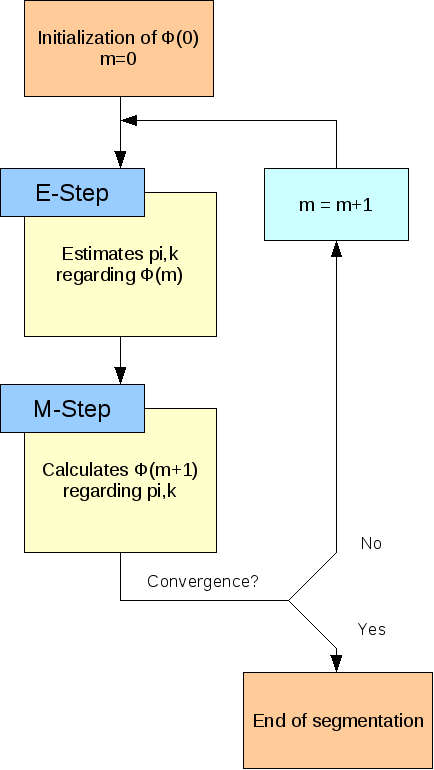
\includegraphics[width=4cm]{Images/Graphics/EMSimple.png}
 \end{center}
}

\subsection{EM segmentation dans Slicer 3}
\frame{ \frametitle{EM segmentation dans Slicer 3}
  \begin{block}{Informations suppl\'ementaires} 
    \begin{itemize}[<+->]      
      \item Atlas probabilistes
      \item Segmentation multi-canaux
      \item Correction des inhomog\'einit\'es de l'intensit\'e
      \item Information hi\'erarchique
    \end{itemize}

  \end{block} 
    

  \begin{center}
 \includegraphics<1>[width=4cm]{Images/Screenshots/atlasT1.png}

 \includegraphics<2>[width=4cm]{Images/Screenshots/T1ForLabel.png}
 \includegraphics<2>[width=4cm]{Images/Screenshots/T2ForLabel.png}
 
 \includegraphics<3>[width=4cm]{Images/Screenshots/T1SagittalNotCorrected.png}
 \includegraphics<3>[width=4cm]{Images/Screenshots/T1SagittalCorrected.png}
  
 \includegraphics<4>[width=4cm]{Images/Graphics/treeStructure.png}
 \end{center} 
  
  
}
\frame{ \frametitle{Processus de segmentation dans Slicer 3}  
  \begin{center}
 \includegraphics<1>[width=10cm]{Images/Graphics/previousalgo.png}
 \end{center} 
}

\frame{\frametitle{Plan}\tableofcontents} 

\section{Contributions} 
\subsection{Initialisation des tissus \`a segmenter}
\frame{\frametitle{Initialisation des tissus \`a segmenter}
  \begin{alertblock}{Pr\'esentation du probl\`eme} 
  M\'ethodes actuelles d'initialisation
    \begin{itemize}[<+->]      
      \item Manuelle : dur \`a estimer
      \item Semi-automatique : peu repr\'esentatif du tissu et non reproductible
    \end{itemize}

  \end{alertblock} 
  }
  
 \frame{\frametitle{Initialisation des tissus \`a segmenter}
    \begin{block}{Solution propos\'ee} 

    \begin{itemize}[<+->]  
      \item Initialisation \`a l'aide d'une "labelmap"    
      \item Repr\'esentatif du tissu \`a segmenter
      \item Reproductible
    \end{itemize}
  \end{block}
  
         \begin{center}
 \includegraphics[width=10cm]{Images/Screenshots/labelmaps.png}
 \end{center} 
}

 \frame{\frametitle{Initialisation des tissus \`a segmenter}
    \begin{exampleblock}{\'Evaluation des r\'esultats} 
    Comparaison Semi-automatique/labelmap
    \begin{itemize}[<+->]  
      \item Initialisation \`a l'aide d'une "labelmap"    
      \item Repr\'esentatif du tissu \`a segmenter
    \end{itemize}
  \end{exampleblock}
  
}

\subsection{\'Evaluation de la s\'election des tissus}
\frame{\frametitle{\'Evaluation de la s\'election des tissus}
  \begin{alertblock}{Pr\'esentation du probl\`eme} 
  M\'ethodes actuelles d'initialisation
    \begin{itemize}[<+->]      
      \item Manuelle : dur \`a estimer
      \item Semi-automatique : peu repr\'esentatif du tissu et non reproductible
    \end{itemize}

  \end{alertblock} 
  }
  
 \frame{\frametitle{\'Evaluation de la s\'election des tissus}
    \begin{block}{Solution propos\'ee} 

    \begin{itemize}[<+->]  
      \item Initialisation \`a l'aide d'une "labelmap"    
      \item Repr\'esentatif du tissu \`a segmenter
      \item Reproductible
    \end{itemize}
  \end{block}
  
         \begin{center}
 \includegraphics[width=10cm]{Images/Screenshots/labelmaps.png}
 \end{center} 
}

 \frame{\frametitle{Initialisation des tissus \`a segmenter}
    \begin{exampleblock}{\'Evaluation des r\'esultats} 
    Comparaison Semi-automatique/labelmap
    \begin{itemize}[<+->]  
      \item Initialisation \`a l'aide d'une "labelmap"    
      \item Repr\'esentatif du tissu \`a segmenter
    \end{itemize}
  \end{exampleblock}
  
}

\subsection{Correction des inhomog\'einit\'es d'intensit\'e}
\frame{\frametitle{numbered lists}
\begin{enumerate}
\item Introduction to  \LaTeX  
\item Course 2 
\item Termpapers and presentations with \LaTeX 
\item Beamer class
\end{enumerate}
}
\subsection{\'Evaluation du param\`etre de normalisation}
\frame{\frametitle{numbered lists with pause}
\begin{enumerate}
\item Introduction to  \LaTeX \pause 
\item Course 2 \pause 
\item Termpapers and presentations with \LaTeX \pause 
\item Beamer class
\end{enumerate}
}
\subsection{\'Evaluation des param\`etres hi\'erarchiques}
\frame{\frametitle{numbered lists with pause}}

\frame{\frametitle{Plan}\tableofcontents} 

\section{Resultats} 
\subsection{Segmentation sans contribution}
\frame{\frametitle{Tables}
\begin{tabular}{|c|c|c|}
\hline
\textbf{Date} & \textbf{Instructor} & \textbf{Title} \\
\hline
WS 04/05 & Sascha Frank & First steps with  \LaTeX  \\
\hline
SS 05 & Sascha Frank & \LaTeX \ Course serial \\
\hline
\end{tabular}}

\subsection{Segmentation apr\`es correction des inhomog\'einit\'es d'intensit\'e}
\frame{\frametitle{Tables with pause}
\begin{tabular}{c c c}
A & B & C \\ 
\pause 
1 & 2 & 3 \\  
\pause 
A & B & C \\ 
\end{tabular} }


\subsection{Segmentation avec la nouvelle m\'ethode d'initialisation des tissus}
\frame{\frametitle{blocs}

\begin{block}{title of the bloc}
bloc text
\end{block}

\begin{exampleblock}{title of the bloc}
bloc text
\end{exampleblock}


\begin{alertblock}{title of the bloc}
bloc text
\end{alertblock}
}

\section{Perspectives}
\frame{\frametitle{blocs}

}
\end{document}

